\documentclass[a4 paper]{article}
% Set target color model to RGB
\usepackage[inner=1.5cm,outer=1.5cm,top=2.5cm,bottom=2.5cm]{geometry}
\usepackage{setspace}
\usepackage[rgb]{xcolor}
\usepackage{verbatim}
\usepackage{amsgen,amsmath,amstext,amsbsy,amsopn,tikz,amssymb,tkz-linknodes}
\usepackage{fancyhdr}
\usepackage[colorlinks=true, urlcolor=blue,  linkcolor=blue, citecolor=blue]{hyperref}
\usepackage[colorinlistoftodos]{todonotes}
\usepackage{rotating}
%\usetikzlibrary{through,backgrounds}
\hypersetup{%
pdfauthor={Arman Shokrollahi},%
pdftitle={Homework},%
pdfkeywords={Tikz,latex,bootstrap,uncertaintes},%
pdfcreator={PDFLaTeX},%
pdfproducer={PDFLaTeX},%
}
%\usetikzlibrary{shadows}
\usepackage[francais]{babel}
\usepackage{booktabs}
\newcommand{\ra}[1]{\renewcommand{\arraystretch}{#1}}

      \newtheorem{thm}{Theorem}[section]
      \newtheorem{prop}[thm]{Proposition}
      \newtheorem{lem}[thm]{Lemma}
      \newtheorem{cor}[thm]{Corollary}
      \newtheorem{defn}[thm]{Definition}
      \newtheorem{rem}[thm]{Remark}
      \numberwithin{equation}{section}

\newcommand{\homework}[6]{
   \pagestyle{myheadings}
   \thispagestyle{plain}
   \newpage
   \setcounter{page}{1}
   \noindent
   \begin{center}
   \framebox{
      \vbox{\vspace{2mm}
    \hbox to 6.28in { {\bf\hfill} }
       \vspace{6mm}
       \hbox to 6.28in { {\Large \hfill #1 (#2)  \hfill} }
       \vspace{6mm}
       \hbox to 6.28in { {\it Instructor: #3 \hfill Student: #5} }
       %\hbox to 6.28in { {\it TA: #4  \hfill #6}}
      \vspace{2mm}}
   }
   \end{center}
   \markboth{#5 -- #1}{#5 -- #1}
   \vspace*{4mm}
}

\newcommand{\bbF}{\mathbb{F}}
\newcommand{\bbX}{\mathbb{X}}
\newcommand{\bI}{\mathbf{I}}
\newcommand{\bX}{\mathbf{X}}
\newcommand{\bY}{\mathbf{Y}}
\newcommand{\bepsilon}{\boldsymbol{\epsilon}}
\newcommand{\balpha}{\boldsymbol{\alpha}}
\newcommand{\bbeta}{\boldsymbol{\beta}}
\newcommand{\0}{\mathbf{0}}

\begin{document}
\homework{Actividad \#6}{Periodo del P\'endulo}{Carlos Liz\'arraga Celaya}{}{Antonio Cota Rodr\'iguez}{}

\section*{Introducci\'on}
\setlength{\parindent}{1.2em}

Como ya vimos en nuestra primera actividad, la matem\'atica del p\'endulo es un poco complicada ya que nos queda por resolver una ecuaci\'on diferencial de segundo orden no lineal hom\'ogenea:

$$ \frac{d^{2}\theta}{dt^{2}} + \frac{g}{l}\sin{\theta} = 0 $$

y ya se ha visto que podemos resolver la ecuaci\'on anterior haciendo que $\sin{\theta} \approx \theta $ esto significa que consideraremos solo oscilaciones peque\~{n}as, esto nos lleva a que la soluci\'on queden en t\'erminos de funciones elementales:

$$\theta(t) = A\cos{(\omega t + \delta)} \quad \quad \quad A\ll 1 $$ 

donde esta es la ya conocida ecuaci\'on del oscilador arm\'onico, con periodo de oscilaci\'on:

$$ T_{0} = 2\pi \sqrt[]{\frac{l}{g}} $$ 

Pero lo que nos concierne ahora es estudiar la soluci\'on de la ecuaci\'on diferencial para {\bf{amplitudes arbitrarias}} (ve\'ase actividad 1 "Deducci\'on de la ecuaci\'on por el m\'etodo de la energ\'ia"), tenemos la siguiente ecuaci\'on diferencial:

$$\frac{d\theta}{dt} =  \sqrt[]{\frac{2g (\cos{\theta}-\cos{\theta_{0}})}{l}}$$

Se invierte la ecuaci\'on y se integra sobre un ciclo completo, as\'i nos queda resolver la siguiente integral:

$$ T = 4\sqrt[]{\frac{l}{2g}}\int_{0}^{\theta_{0}}\frac{d\theta}{\sqrt[]{(\cos{\theta}-\cos{\theta_{0}})}} $$

Obteni\'endo el cociente de los dos periodos $T/T_{0}$ nos da la desviaci\'on del periodo verdadero del p\'endulo para una aproximaci\'on de oscilaciones peque\~{n}as.

\begin{figure}[!ht]
  \centering
      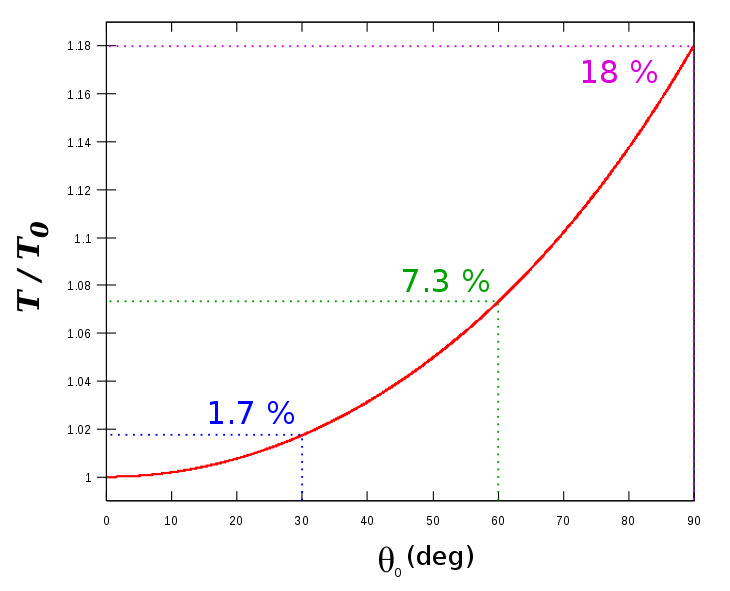
\includegraphics[width=7cm, height=6cm]{PeriodoVerdadero.png}
  \caption{Desviaci\'on para peque\~{n}as oscilaciones}
\end{figure}

notar que $\lim_{\theta_{0}\to \pi} T = \infty$.

\newpage

\section*{Programa}

En esta actividad se realiz\'o un c\'odigo en ipython con objetivo de resolver la integral para el periodo del p\'endulo con un error m\'inimo as\'i relacionando en una gr\'afica el error relativo y $\theta_{0}$.

\begin{verbatim}

# Paquetes
import numpy as np
from scipy import integrate
import matplotlib.pyplot as plt


# Numero de angulos a integrar
n=1000

# Arreglos, tomando error de 0.0001
x=[]
TT0=[]
x_0=np.linspace(0.0001,np.pi + 0.0001, n)



# La funcion a integrar
I = lambda x,a: 1/np.sqrt(np.cos(x) - np.cos(a))


for i in range(n):
# Integral
    theta_0=x_0[i]
    T , err= integrate.quad(I, 0, theta_0, args=(theta_0,))
    
    
# Error
    TT0.append(np.sqrt(2)/np.pi * T)
    
    
    
# Graficas
plt.figure(1)
plt.plot(x_0 * 180 / np.pi, TT0 , "r" )
plt.title('Desviacion')
plt.xlabel(r'$ \theta _0 (grados)$')
plt.ylabel("T/To")
plt.xlim(0,90)
plt.ylim(1,1.2)
plt.grid()

plt.show()

plt.figure(1)
plt.plot(x_0 * 180 / np.pi, TT0 , "b" )
plt.title('Divergencia en ' r'$\theta_0 = \pi$')
plt.xlabel(r'$ \theta _0 (grados)$')
plt.ylabel("T/To")
plt.xlim(0,180)
plt.ylim(1,5)
plt.grid()


plt.show()


\end{verbatim}

Para $n=1000$ y $\epsilon = 0.0001$ obtuvimos las siguientes gr\'aficas:

\begin{figure}[!ht]
  \centering
      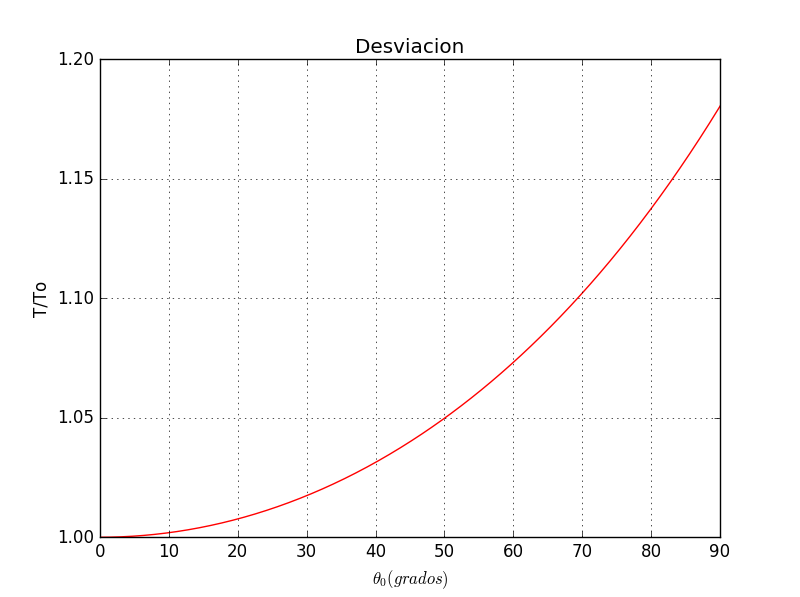
\includegraphics[width=7cm, height=6cm]{Desviacion.png}
  \caption{}
\end{figure}

\vspace*{0.5cm}

\begin{figure}[!ht]
  \centering
      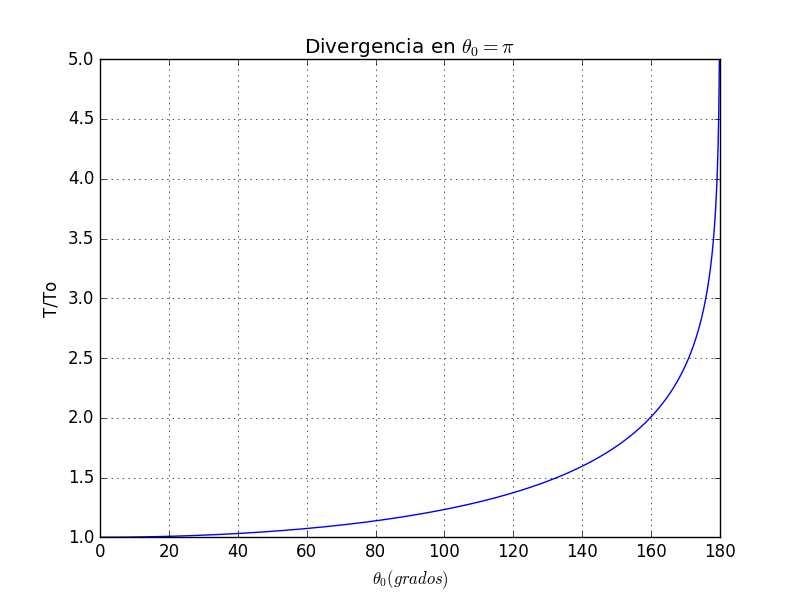
\includegraphics[width=7cm, height=6cm]{Divergencia.png}
  \caption{}
\end{figure}

\section*{Conclusi\'on}
Pudimos comprobar gr\'aficamente como diverge $T/T_{0}$ cuando $\theta \rightarrow \pi$ utilizando el m\'etodo para integrar de {\bf scipy.integrate.quad}.


\end{document}